\documentclass[11pt, abstract=on]{scrartcl}
\usepackage[formal]{tengwarscript}
\pdfmapfile{=tengwarscript.map}
\usepackage{amsmath,amssymb,amsfonts}
\usepackage{algorithmic}
\usepackage[utf8]{inputenc}
\usepackage[T1]{fontenc}
\usepackage[ngerman]{babel}

\usepackage{hyperref}
\usepackage{graphicx} 

\usepackage{listings}

\def\BibTeX{{\rm B\kern-.05em{\sc i\kern-.025em b}\kern-.08em
    T\kern-.1667em\lower.7ex\hbox{E}\kern-.125emX}}

\begin{document}
\lstset{language=[11]C++}   

\begin{abstract}

This work introduces a way to generate ``plants'', espe
\end{abstract}

\section{Einführung und Allgemeines}
In diesem Praktikum sollen verschiedene Werte gemessen werden. 

Grundlage CPU (Host) und GPU (Client)

Einige relevante Spezifikationen der Grafikkarte sind:
\begin{itemize}
	\item 1920 Cores, wovon ein Warp jeweils 32~Threads umfasst
	\item Maximale Taktung laut "`nvidia-smi"': 1708 MHz
	\item Speicherkonfiguration: 8 GB GDDR5~RAM
	\item Herstellerangabe für den Durchsatz: 256~GB/s
	\item PCIe~3.0 fähig, in der Messung wurde allerdings nur PCIe 2.0x16 verwendet. Die maximale Kopierrate von PCIe 2.0x16 entspricht 8.0GB/s
\end{itemize}

Grundlage CPU (Host) und GPU (Client) 

Als Vergleichsmaßstab für die unterschiedlichen Kernel ist zuerst die mit Standard-Kopieroperatoren erziehlbare Kopierrate relevant. Abbildung~\ref{fig:Kopierrate} zeigt die für \texttt{CudaMalloc()} gemessenen Kopierraten und die vom Hersteller angegebenen Maximalwerte sowie die Spezifikation für den verwendeten PCIe.

\begin{figure} [htbp]
 	\centering
 		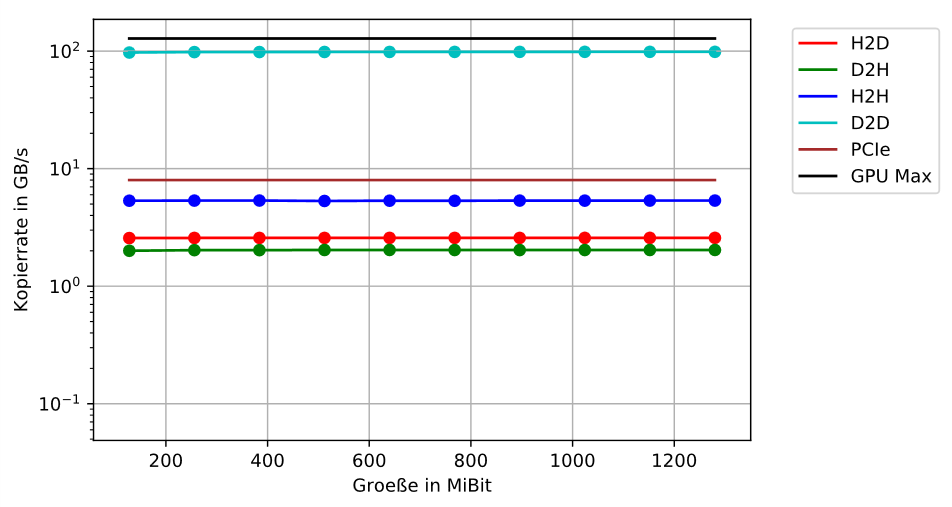
\includegraphics[width=0.7\textwidth]{Graph_Kopierrate.png}
 	\caption{Kopierrate von CudaMemcpy()}
 	\label{fig:Kopierrate}
\end{figure}

Bei der tatsächlichen Durchführungen der Messungen ist es wichtig, zu beachten, dass jeweils der erste Kernel Aufruf eines CUDA Programms eine wesentlich längere Zeit benötigt als darauf folgende Aufrufe des selben Kernels. Abbildung~\ref{fig:StartupCost} zeigt eine Beispielmessung für einen Empty Kernel, dh. einen Kernel, der zwar aufgerufen wird, dann auf der GPU allerdings keine Arbeit verrichtet. Um dieser Verzerrung entgegenzuwirken, muss vor jeder Laufzeitmessung für einen Kernel dieser einmal als "`Warmup"' aufgerufen, aber dann aus der eigentlichen Messung herausgerechnet werden.

\begin{figure} [htbp]
 	\centering
 		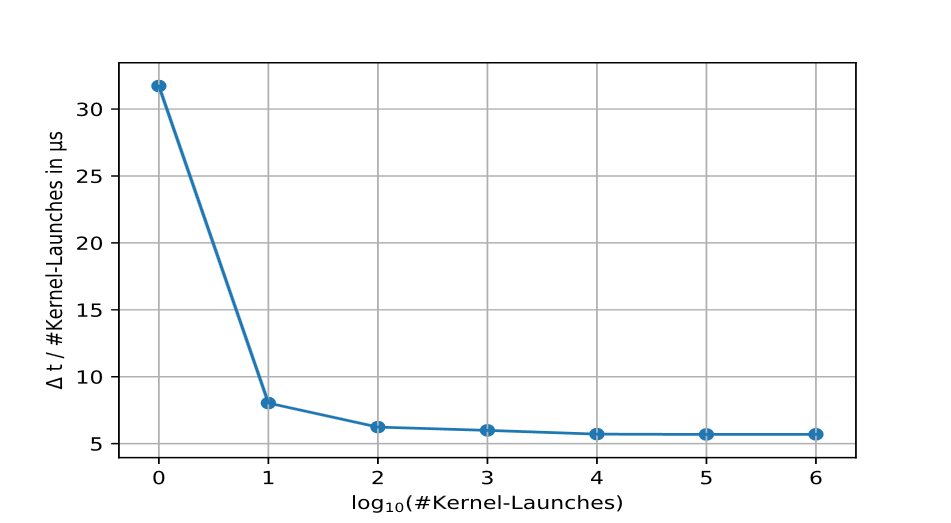
\includegraphics[width=0.7\textwidth]{Graph_Startup.png}
 	\caption{Startup Cost eines Empty Kerneles}
 	\label{fig:StartupCost}
\end{figure}

\section{Copy Kernel}

Der "`Copy Kernel"', der jeweils ein Element eines Buffers in die entsprechende Position eines anderen Buffers kopiert, lässt sich durch folgenden CUDA-Quellcode beschreiben:

\begin{lstlisting} 
template<typename T>
__global__
void copyKernel(T* out, T* in) {
	unsigned id = threadIdx.x + blockIdx.x * blockDim.x;
		
	out[id] = in[id];
}
\end{lstlisting}

Obwohl die Funktion als Input nur Zeiger auf ein Quell-und ein Ziel-Buffer nimmt, gibt es doch drei implizite Parameter. Diese treten auch bei allen folgenden Messungen auf:
\begin{enumerate}
	\item Anzahl der Blöcke, in die die einzelnen Threads von der GPU gruppiert werden
	\item Die Größe dieser Blücke
	\item Zugriffstyp \texttt{T} (zB. \texttt{char}, \texttt{int})
\end{enumerate}
 Abbildung~\ref{fig:CopyKernel1} und Abbildung~\ref{fig:CopyKernelBlocks} zeigen die Auswirkungen von Variationen über die drei Parameter auf die durch den Copy Kernel erzielte Kopierrate. Dabei zeigt sich, dass sowohl für die Anzahl der Blöcke, für die Blockgröße als auch für \texttt{sizeof(T)} ein jeweils höherer Parameter zu einer besseren Kopierrate führt. Für hinreichend hohe Werte wird eine Sättigung nahe des Ergebnisses aus Abbildung~\ref{fig:Kopierrate} erzielt. Interessant ist außerdem, dass die Abbildungen sich mit steigendem \texttt{sizeof(T)} je linearer verhalten, je geringer Blockgröße bzw. Blockanzahl sind.

\begin{figure} [htbp]
 	\centering
 		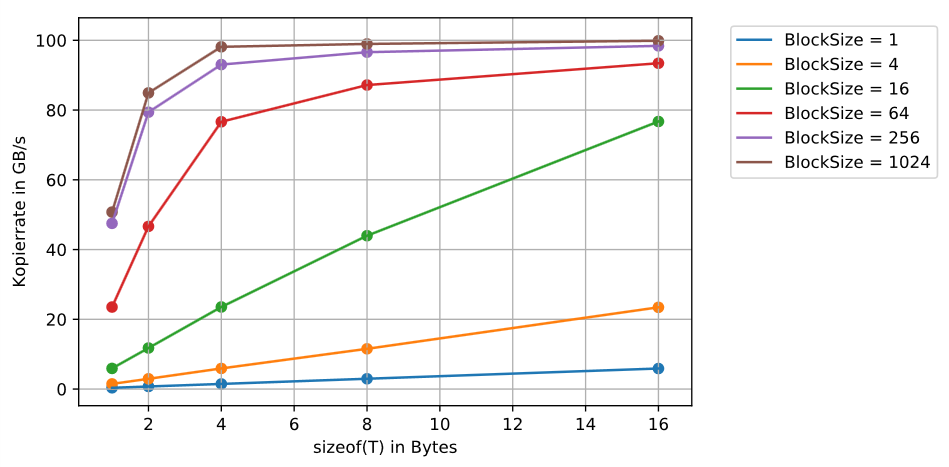
\includegraphics[width=0.7\textwidth]{Graph_CopyKernel1.png}
 	\caption{Variation über \texttt{BlockSize} und \texttt{sizeof(T)}, $\texttt{numBlocks} = 16384$}
 	\label{fig:CopyKernel1}
\end{figure}

\begin{figure} [htbp]
 	\centering
 		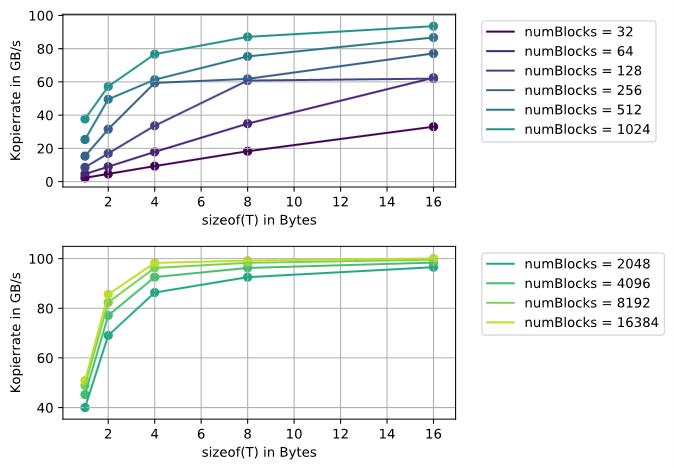
\includegraphics[width=0.7\textwidth]{Graph_CopyKernelBlocks.png}
 	\caption{Variation über \texttt{numBlocks} und \texttt{sizeof(T)}, $\texttt{BlockSize} = 1024$}
 	\label{fig:CopyKernelBlocks}
\end{figure}

\section{Strided Access}
Der Strided Access ist wie folgt definiert:

\begin{lstlisting} 
template<typename T>
__global__
void copyKernel(T* out, T* in, int stride) {
	unsigned id = threadIdx.x + blockIdx.x * blockDim.x;
		
	out[id*stride] = in[id*stride];
}
\end{lstlisting}

Das heißt, der Zugriff erfolgt nicht mehr auf jedes Element konsekutiv hintereinander, sondern nur auf jedes $N$-te Element. Zusätzlicher Parameter ist dann der \texttt{stride}, der festlegt, wie viele Buffer-Einträge übersprungen werden. Bei elementarem Zugriff, wie er zum Beispiel in einer Turingmaschine definiert ist, sollte sich keine Änderung der Kopierrate ergeben, sofern die nicht bearbeiteten Elemente nicht mitgerechnet werden. Beim der Messung zeigt sich aber, dass deutliche Cashe-Effekte auftreten. Bei Messungen zeigt sich ein nahezu exponentieller Abfall der Kopierrate mit steigendem \texttt{stride}, für den die beiden Messungen Abbildung~\ref{fig:StridedAccess1} und Abbildung~\ref{fig:StridedAccess2} beispielhaft stehen. Bei $\texttt{sizeof(T)} \cdot \texttt{stride} = 32$ und $\texttt{sizeof(T)} \cdot \texttt{stride} = 64$ ergeben sich jeweils zwei fast gleiche Werte, und ab $\texttt{sizeof(T)} \cdot \texttt{stride} = 2048$ fällt die Kopierrate wenn überhaupt nur noch vernachlässigbar ab (bei diesen beiden Messungen wie auch bei allen anderen).

\begin{figure} [htbp]
 	\centering
 		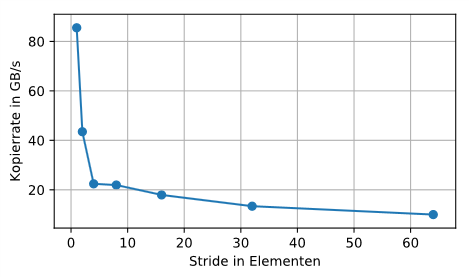
\includegraphics[width=0.7\textwidth]{Graph_StridedAccess1.png}
 	\caption{Strided Access: Variation über \texttt{stride}, $\texttt{BlockSize} = 256$, $\texttt{numBlocks} = 4096$, \texttt{T}:~\texttt{int2}~($\texttt{sizeof(int2)} = 8$)}
 	\label{fig:StridedAccess1}
\end{figure}

\begin{figure} [htbp]
 	\centering
 		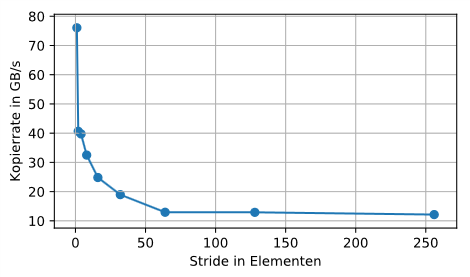
\includegraphics[width=0.7\textwidth]{Graph_StridedAccess2.png}
 	 	\caption{Strided Access: Variation über \texttt{stride}, $\texttt{BlockSize} = 128$, $\texttt{numBlocks} = 2048$, \texttt{T}:~\texttt{int4}~($\texttt{sizeof(int4)} = 16$)}
 	\label{fig:StridedAccess2}
\end{figure}

\section{Offset Access}

\begin{figure} [htbp]
 	\centering
 		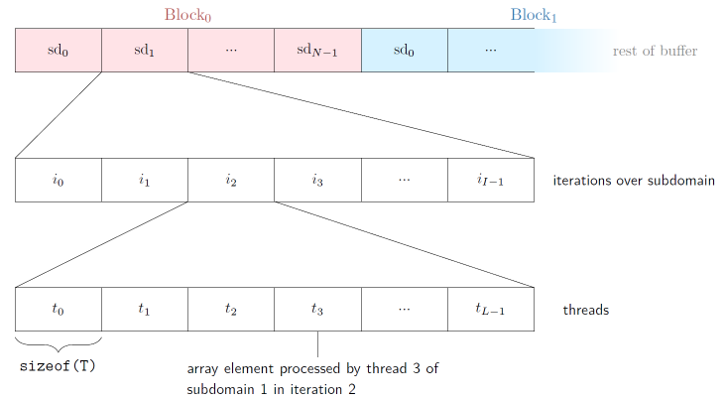
\includegraphics[width=0.7\textwidth]{Graph_OffsetAccessZugriff.png}
 	\caption{}
\end{figure}

\begin{figure} [htbp]
 	\centering
 		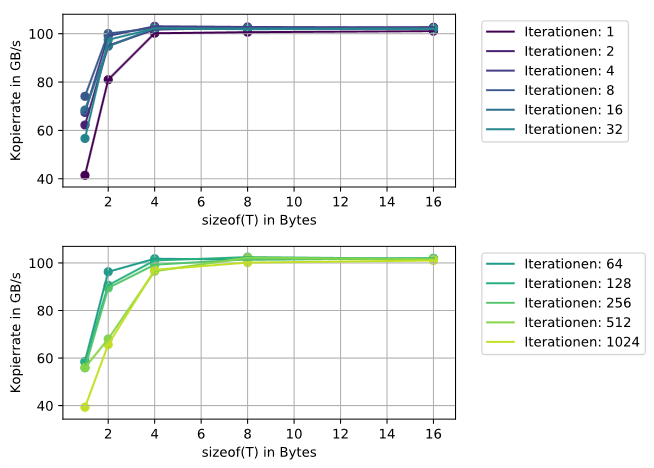
\includegraphics[width=0.7\textwidth]{Graph_OffsetAccess1.png}
 	\caption{}
\end{figure}

\begin{figure} [htbp]
 	\centering
 		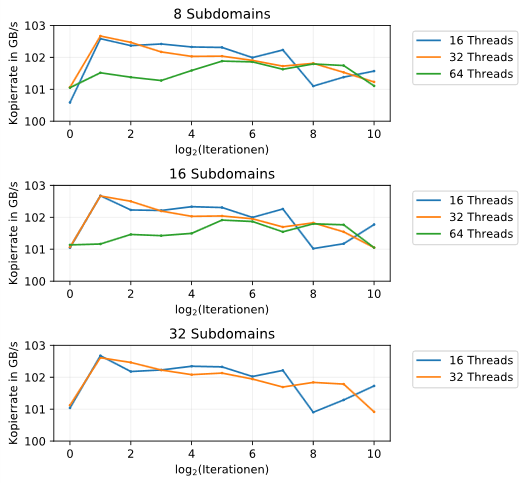
\includegraphics[width=0.7\textwidth]{Graph_OffsetAccessSDpBlock.png}
 	\caption{}
\end{figure}

\begin{figure} [htbp]
 	\centering
 		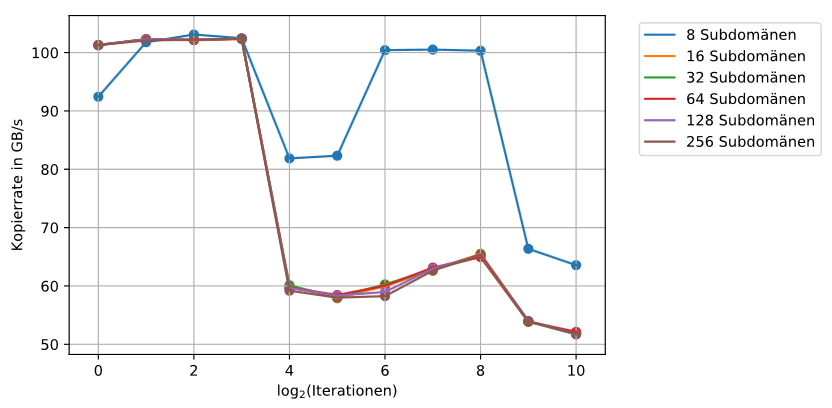
\includegraphics[width=0.7\textwidth]{Graph_OffsetAccessSDpBlock2.png}
 	\caption{}
\end{figure}

\begin{figure} [htbp]
 	\centering
 		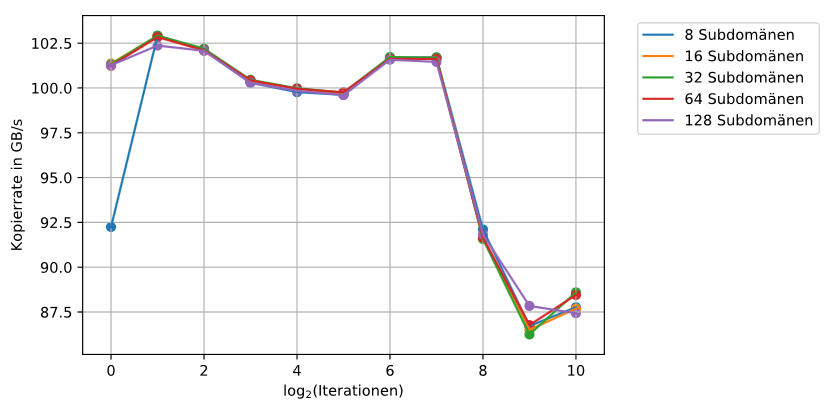
\includegraphics[width=0.7\textwidth]{Graph_OffsetAccessSDpBlock3.png}
 	\caption{}
\end{figure}

\begin{figure} [htbp]
 	\centering
 		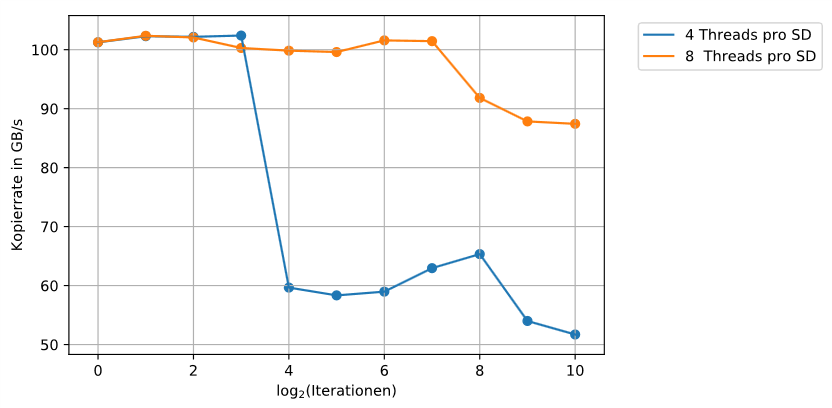
\includegraphics[width=0.7\textwidth]{Graph_OffsetAccessSDpBlock4.png}
 	\caption{}
\end{figure}

\begin{figure} [htbp]
 	\centering
 		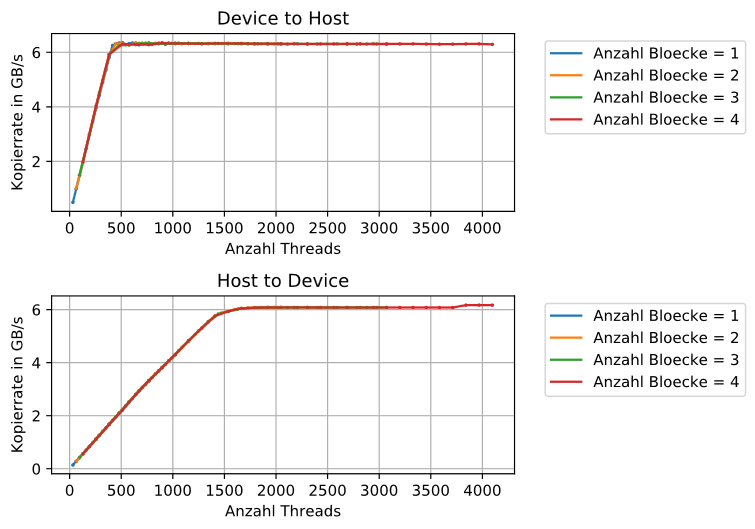
\includegraphics[width=0.7\textwidth]{Graph_CudaMalloc.png}
 	\caption{}
\end{figure}

\begin{figure} [htbp]
 	\centering
 		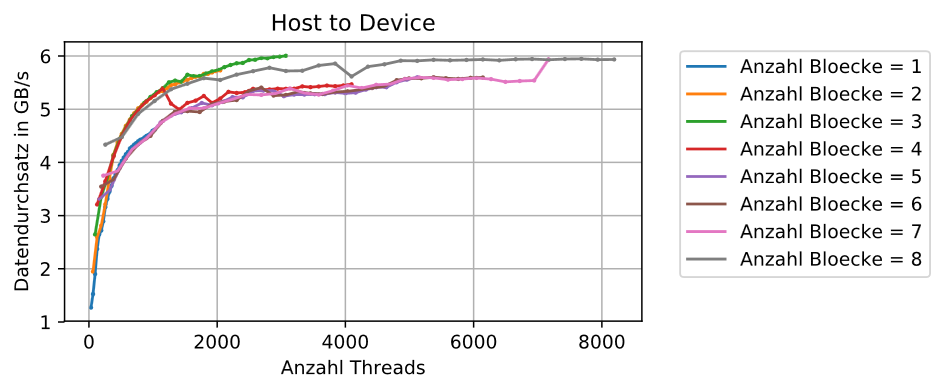
\includegraphics[width=0.7\textwidth]{Graph_CudaMallocManaged.png}
 	\caption{}
\end{figure}

\begin{figure} [htbp]
 	\centering
 		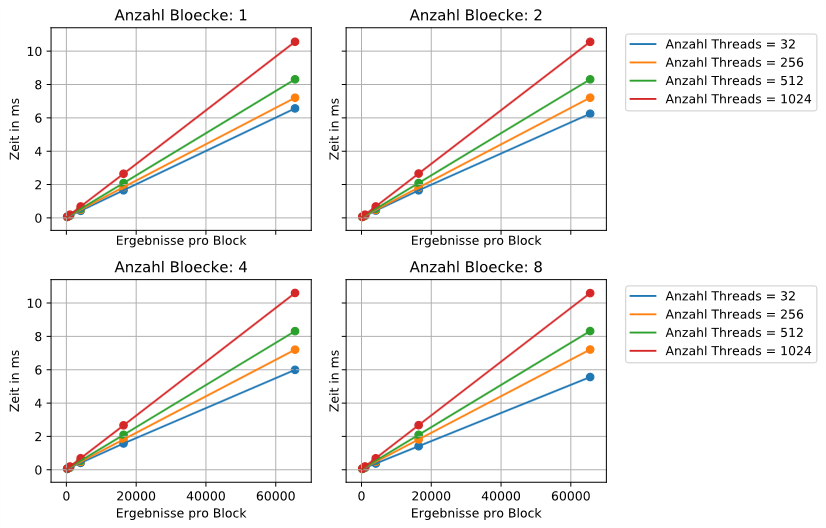
\includegraphics[width=0.7\textwidth]{Graph_KommunikationOhne.png}
 	\caption{}
\end{figure}

\begin{figure} [htbp]
 	\centering
 		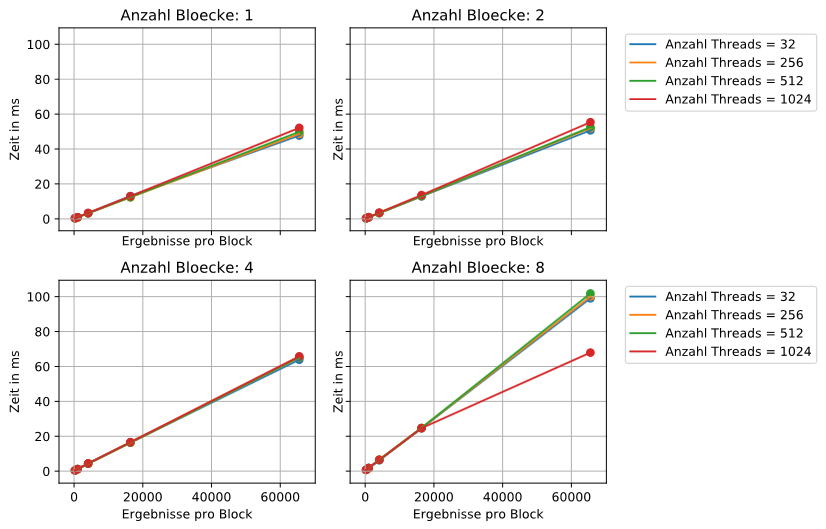
\includegraphics[width=0.7\textwidth]{Graph_KommunikationMit.png}
 	\caption{}
\end{figure}


\begin{figure} [htbp]
 	\centering
 		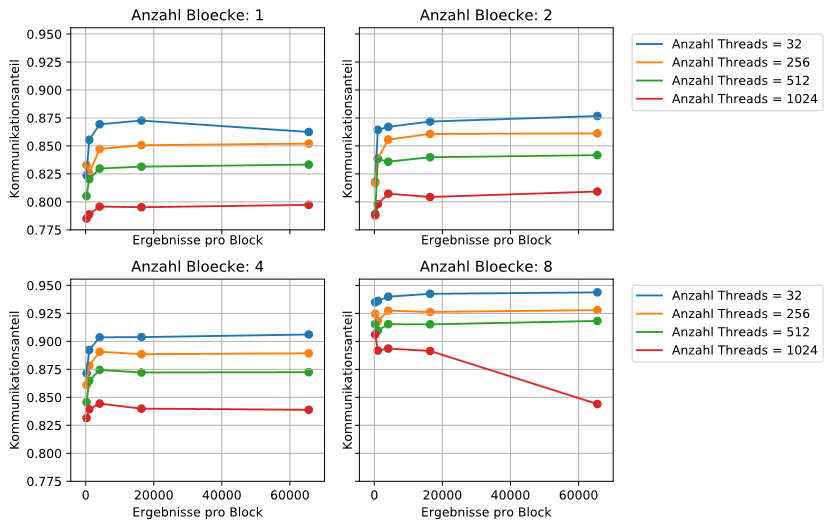
\includegraphics[width=0.7\textwidth]{Graph_KommunikationAnteil.png}
 	\caption{}
\end{figure}

\begin{thebibliography}{99}
	\bibitem{WikipediaDogRose}  \href{https://commons.wikimedia.org/wiki/File:Hundsrose.jpg}{Wikimedia: ``Hundsrose.jpg'', commons.wikimedia.org/wiki/File:Hundsrose.jpg}, viewed on 01/13/19
	\bibitem{WikipediaTree} \href{https://commons.wikimedia.org/wiki/File:Baum_im_Sossusvlei.jpg}
	{Wikimedia: ``Baum im Sossusvlei.jpg'', commons.wikimedia.org/wiki/File:Baum\_ im\_Sossusvlei.jpg}, viewed on 01/13/19
	\bibitem{WhatIsUnreal}  \href{https://www.unrealengine.com/en-US/what-is-unreal-engine-4}{``Make Something Unreal'', unrealengine.com/en-US/what-is-unreal-engine-4}, viewed on 01/13/19
	\bibitem{MinecraftTree}  \href{https://minecraft.gamepedia.com/Tree}{Minecraft Wiki: ``Tree', minecraft.gamepedia.com/Tree}, viewed on 01/13/19
	\bibitem{Spore}  \href{https://en.wikipedia.org/wiki/Spore_(2008_video_game)}{Wikipedia: ``Spore', en.wikipedia.org/wiki/Spore\_(2008\_video\_game)}, viewed on 01/13/19
	\bibitem{CellLab}  \href{http://cell-lab.net/}{Cell Lab website, cell-lab.net/}, viewed on 01/13/19
	\bibitem{EcoGame}  \href{https://www.strangeloopgames.com/eco/}{Eco website, strangeloopgames.com/eco/}, viewed on 01/13/19
	\bibitem{SpeedTree}  \href{https://store.speedtree.com/}{SpeedTree website, store.speedtree.com/}, viewed on 01/13/19
	\bibitem{UEInstancing}  \href{https://api.unrealengine.com/INT/API/Runtime/Engine/Components/UInstancedStaticMeshComponent/index.html}{UE API Documentation (api.unrealengine.com/): ``UInstancedStaticMeshComponent''}, viewed on 01/13/19
	\bibitem{UESplines}  \href{https://docs.unrealengine.com/en-us/Engine/BlueprintSplines/Overview}{UE Documentation (docs.unrealengine.com/en-us/): ``Blueprint Spline Components Overview''}, viewed on 01/13/19
	\bibitem{ClimbingPlants}  \href{http://www.cse.chalmers.se/~uffe/xjobb/climbingplants.pdf}{Johan Knutzen, ``Generating Climbing Plants Using L-Systems''}, viewed on 01/13/19
	
\end{thebibliography}
\end{document}

